\documentclass[a4paper]{oblivoir}
\author{Moon Il-chul \\ \href{mailto:icmoon@kaist.ac.kr}{icmoon@kaist.ac.kr} 
   \and Shin Seung-jae \\ \href{mailto:tmdwo0910@kaist.ac.kr}{tmdwo0910@kaist.ac.kr} }
\setcounter{chapter}{13}
\title{Chapter 13. Dirichlet process}
\usepackage{indentfirst}
\usepackage{graphicx}
\graphicspath{ {Figure/} }
\usepackage{hyperref}
\usepackage{amsmath}
\usepackage{amssymb}
\usepackage{amsfonts}
\usepackage{dsfont}
\usepackage[]{algorithm2e}
\usepackage{chngcntr}
\counterwithin{figure}{chapter}
\setcounter{tocdepth}{2}
\setcounter{secnumdepth}{3}
\hypersetup{pdfborder={0 0 0}}
\renewcommand{\thefigure}{\thechapter-\arabic{figure}}
\renewcommand{\theequation}{\thechapter.\arabic{equation}}
\newlength\myindent
\setlength\myindent{5em}

\begin{document}
\maketitle
\tableofcontents


%\chapter{}
%-----------------------------------------------------------------
\section{Definition of Dirichlet process}
%-----------------------------------------------------------------
이번 장에서는 Dirichlet process에 대해 알아보도록 하겠다. Dirichlet process는 stochastic process 중 하나로, clustering 기법 적용시 cluster 개수인 k를 추정할 때 사용되는 방법론이자 과정이다. 즉, 사람이 임의로 cluster의 개수를 정할 때 생길 수 있는 문제를 해결하는 데 도움을 주는 개념이라 할 수 있다. 

\subsection{Detour: Gaussian Mixture model}
%-----------------------------------------------------------------
Dirichlet process를 정의하기 전에 clustering model 중 우리가 배운 바 있는 Gaussian mixture model에 대해 다시 한번 이야기해보도록 하겠다. 

\begin{figure}[ht] \centering 
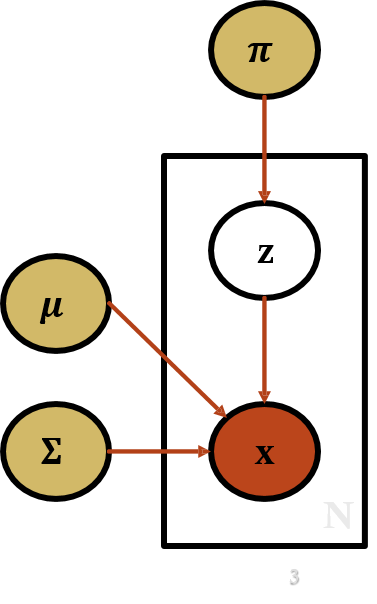
\includegraphics[scale=0.4]{fig13_1.png} 
\caption{graphical model of GMM}
\label{fig:13-1}
\end{figure}

위의 그림은 GMM을 표현한 것이다. 먼저 graphical model에 표현된 변수와 파라미터에 대해 알아보도록 하겠다. 첫번째로 x는 우리에게 주어진 data를 의미하며 $\mu$와 $\sum$의 경우 각 클러스터의 centroid를 나타내는 parameter들이라 할 수 있다. 또한, 각 클러스터마다 centroid는 하나씩 존재하기 때문에 $\mu$, $\sum$은 k개의 cluster에 대해 k개 만큼의 값을 가지게 된다. z의 경우 각각의 data에 대한 cluster assignment를 결정하는 multinomial distribution에 대한 변수이라고 할 수 있으며 z에 영향을 주는 $\pi$의 경우 각  cluster의 분포, 즉 각각의 데이터가 각 cluster에 포함되는 비율을 결정짓는 parameter라고 할 수 있다. 고로 $\pi$의 dimension 또한 k가 된다. 

결국 centroid 개수와 클러스터의 개수를 결정짓는 중요한 키는 k라는 것을 변수와 파라미터를 통해 알 수 있다. 변수와 파라미터의 특성을 고려하여 P(x)를 표현하면 아래와 같다. 
\begin{equation}
P(x) = \sum^{K}_{k=1}P(z_{k})P(x|z) =
\sum^{K}_{k=1}\pi_{k}N(x|\mu_{k},{\Sigma}_{k})
\label{eq:13-2-1}
\end{equation}

1. mixing coefficient, or Selection variable $z_{k}$
\begin{equation}
z_{k} \in \{0,1\}, \; \sum^{K}_{k=1}z_{k} = 1, \; P(z_{k}=1) = \pi_{k}, \; \sum^{K}_{k=1}\pi_{k} = 1, \; 0 \leq \pi_{k} \leq 1, \,
P(z) = \prod^{K}_{k=1}\pi^{z_{k}}_{k} \nonumber \\
\end{equation}

2. mixture component
\begin{equation}
P(X|z_{k}=1) = N(x|\mu_{k},\Sigma _{k})\; \rightarrow \; p(X|Z) = \prod^{K}_{k=1}N{(x|\mu_{k},{\Sigma}_{k})}^{z_{k}}\nonumber \\
\end{equation}

위에서 볼 수 있듯이 cluster의 개수이자 Choice size인 k는 모든 parameter 및 변수에 영향을 미치는 매우 중요한 값이다. 고로 k의 값를 자유롭게 조정하고 변화시키는 것이 cluster model에 매우 중요한 요소임을 알 수 있다.

\subsection{Detour: Dirichlet Distribution}
%-----------------------------------------------------------------
위의 장을 통해 Gaussian mixture model의 변수 z가 multinomial distribution을 따른다는 것을 알 수 있었고, 또한 z는 parameter $\pi$에 의해 영향을 받는다는 것을 알 수 있었다. 이 때, z의 multinomial distribution 또한 자유로운 제어와 조정이 필요해짐을 알 수 있다.  각각의 multinomial distribution마다 parameter $\pi$를 임의로 조정해주는 것은 매우 비효율적이기 때문이다. 아울러 이는 최종적인 목적이라고 할 수 있는 cluster 개수 k의 제어를 위해서도 꼭 필요한 과정이라 할 수 있다.

이렇듯 multinomial distribution을 다양한 값과 조건으로 생성 및 조정할 수 있는 수단으로 우리는 Dirichlet distribution을 활용하기로 한다. 

아래의 LDA (Latent Dirichlet allocation) 모델 예시를 통하여 Dirichlet distribution에 대해 설명해보도록 하겠다.

\begin{figure}[ht] \centering 
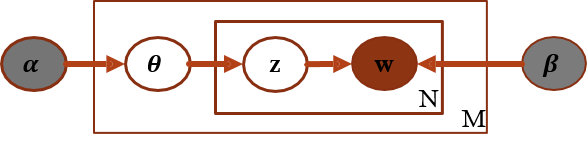
\includegraphics[scale=0.5]{fig13_2.png} 
\caption{graphical model of LDA}
\label{fig:13-2}
\end{figure}

* Generative Process
\begin{equation}
\begin{split}
\theta_{t} \sim Dir(\alpha), \; t \in \{1,...,M\}, \; k \in \{1,...,K\} \\
z_{i,l} \sim Multi(\theta_{i}), \; l \in \{1,...,M\}, \; i \in \{1,...,M\}, \; l \in \{1,...,N\} \nonumber
\end{split}
\end{equation}

위와 같이 dirichlet distribution의 $\alpha$에 의해 sampling된 $\theta_{i}$의 경우 multinomial distribution인 z의 parameter로 들어갈 수 있다. 왜냐하면 dirichlet distribution은 각각의 변수가 probability axiom을 만족하는 형태로 존재하며 이는 multinomial distribution의 parameter로 매우 적절한 형태이기 때문이다. 이러한 dirichlet distribution의 특성을 통해 multinomial distribution의 parameter에 대한 조정이 가능해짐을 알 수 있다. 아래는 dirichlet distribution에 대한 설명이다.\\


* dirichlet distribution
\begin{eqnarray*}
&P(x_{1},...,x_{K}|\alpha_{1},...,\alpha_{K}) = \frac{\Gamma(\sum^{K}_{i=1}\alpha_{i})}{\Pi^{N}_{i=1}\Gamma(\alpha_{i})}{x_{i}}^{\alpha_{i}-1}\nonumber\\
&x_{1},...,x_{K-1} > 0 \\
&x_{1}+...+x_{K-1} < 1 \\
&x_{K}=1-x_{1}-x_{2}-...-x_{K-1}\\
&\alpha_{i} > 0 \; (for 1 \leq i \leq K)
\end{eqnarray*}

\subsection{Multinomial-Dirichlet Conjugate Relation}
%-----------------------------------------------------------------
이번 장에서는  multinomial distribution과 dirichlet distribution간에 정의되는 conjugate relation에 대해 알아보도록 하겠다. 

* Multinomial distribution

\begin{equation}
P(D|\theta) = \frac{N!}{\prod_{i} c_{i}!}\Pi_{i}{\theta_{i}}^{c_{i}} \; \Big(N = \sum_{i}c_{i}, ~ D=(c_{i}) \Big)
\end{equation}

먼저 Multinomial distribution의 경우 N개의 iid (indepedently and identically distributed) instance들에 대하여 위와 같이 정의할 수 있다. 식에서 볼 수 있다시피 $\theta_{i}$에 대한 자승의 형태로 $c_{i}$가 들어감을 알 수 있다.\\

* Dirichlet distribution

\begin{equation}
P(\theta|\alpha) = \frac{1}{B(\alpha)}\Pi_{i}{\theta_{i}}^{\alpha_{i}-1}
\end{equation}

dirichlet distribution의 경우도 normalizer에 대한 부분을 $B(\alpha)$로 나타내줄 경우 위와 같이 표현해줄 수 있다. 여기서 눈여겨볼 점은 dirichlet distribution 또한  $\theta_{i}$에 대한 자승의 형태로 $\alpha_{i}-1$가 들어갔다는 점이다. Multinomial distribution과 매우 비슷한 형태를 가지고 있고 각 distribution에 대한 곱을 할 경우 $\theta_{i}$의 자승인 $c_{i}$과 $\alpha_{i}-1$을 각각 더해주기만 하면 된다는 점에서 dirichlet distribution과 Multinomial distribution은 서로 연산이 매우 편리한 관계임을 알 수 있다.

이를 이용하여 Multinomial distribution의 P(D$|$ $\theta$)를 likelihood로, dirichlet distribution의 P($\theta$$|$$\alpha$)를 prior로 취급할 경우 이에 대한 posterior P($\theta$ $|$D,$\alpha$)를 우리는 다음과 같이 정의할 수 있다.\\

* Bayesian Posterior
\begin{eqnarray}
P(\theta|D,\alpha) & \propto &  P(D|\theta)P(\theta|\alpha) = \frac{N!}{\Pi_{i} c_{i}!}\Pi_{i}{\theta_{i}}^{c_{i}}\frac{1}{B(\alpha)}\Pi_{i}{\theta_{i}}^{\alpha_{i}-1}\nonumber \\
& = & \frac{N!}{B(\alpha)\Pi_{i}c_{i}!}\Pi_{i}
{\theta_{i}}^{\alpha_{i}+c_{i}-1} \propto \Pi_{i}
{\theta_{i}}^{\alpha_{i}+c_{i}-1}
\end{eqnarray}

즉, posterior distribution인  $P(\theta|D,\alpha)$ 또한 dirichlet distribution의 꼴로 나타내어짐을 알 수 있다. dirichlet distribution의 normalizer 영역까지 함께 고려하여 posterior distribution의 식을 완성하면 다음과 같다. 

\begin{equation}
P(\theta|D,\alpha) = \frac{1}{B(\alpha+c)}\Pi_{i}
{\theta_{i}}^{\alpha_{i}+c_{i}-1}
\end{equation}

위와 같이 prior distribution과 likelihood function을 통해 정의한 posterior distribution이 prior distribution과 같은 형태가 될 때 이를 conjugate prior라고 정의한다. 

이를 문장으로 표현할 경우 Dirichlet distribution의 likelihood는 multinomial distribution의 conjugate prior이다라고도 이야기할 수 있다. 또한 bayesian posterior distribution은 data를 통해 정의된 likelihood function에 prior belief를 반영한 결과라고 이야기할 수 있는데, 이를 dirichlet distribution의 예시로 설명하면 다음과 같다.\\

* Dirichlet distribution with D as a single observation with i-th choice
\begin{equation}
\theta|\alpha \sim Dir(\alpha_{1},...,\alpha_{i},...,\alpha_{N}) \; \rightarrow \; \theta|D,\alpha \sim Dir(\alpha_{1},...,\alpha_{i} + 1,...,\alpha_{N})
\end{equation}

\subsection{Dirichlet Process}
%-----------------------------------------------------------------
이제 본격적으로 Dirichlet process에 대해 알아보도록 하겠다. 먼저 Dirichlet process는 다음과 같이 정의할 수 있다.\\

* Dirichlet process
\begin{equation}
G|\alpha,H \; \sim \; DP(\alpha,H) 
\end{equation}
\begin{eqnarray}
(G(A_{1}),...,G(A_{r}))|\alpha,H \;&\sim&\; Dir(\alpha H(A_{1}),...,\alpha H(A_{r}))\nonumber\\
A_{i}\cap A_{j} = &\varnothing&,  A_{1}\cup ... \cup A_{r} = \Theta \nonumber
\end{eqnarray}

위의 식에서 볼 수 있듯이 Dirichlet distribution의 parameter로 쓰였던 $\alpha$뿐만 아니라 새로운 형태인 H가 함께 ditribution에 영향을 주고 있음을 알 수 있다. 또한 vector 형태로 introduce된 G의 각 dimension에 해당하는 $A_{i}$의 경우 상호간 배타적인 (mutually exclusive) 관계로 존재한다. 이 때 우리는 Dirichlet distribution의 parameter로 각각 반영된 $H(A_{1})$을 통해 H의 용도를 파악할 수 있다. 바로 mutually exclusive하게 분류된 $A_{i}$(i = 1...r)을 Probability distribution, 즉 확률분포의 형태로 변환시켜주는 데 H의 목적이 있는 것이다. 각각의 값에 대한 합을 1로 만들어줄 수 있다면 mutually exclusive한 각각의 사건을 확률분포로 바꿔준 $H(A_{i})$는 probability axiom을 잘 만족하는 형태가 될 것이다. Dirichlet process가 가지는 평균과 분산은 다음과 같다.\\

* Property of Dirichlet process
\begin{eqnarray}
E[G(A)] = H(A)\;\;,\;\;V[G(A)] =\frac{H(A)(1-H(A))}{\alpha+1}
\end{eqnarray}
\begin{center}
H : Base distribution\\
$\alpha$ : Concentration parameter, strength parameter (strength of prior)
\end{center}

dirichlet process에서 parameter로 쓰인 $\alpha H(A_{i})$에 대해, $\alpha$는 각 parameter의 값에 대한 집중도를 결정짓는다는 점에서 그래프의 모양에는 영향을 주지만 정확한 위치에는 전혀 영향을 주지 않는다. 고로 평균은 H에 의해서만 영향을 받으며 분산의 경우 $\alpha$와 H 둘 모두에 의해 영향을 받게 된다. \\


* Posterior distribution given a dataset of $\theta_{1},...,\theta_{n}$

위에서 설명한 Dirichlet process에 대한 정의를 바탕으로 n개의 data가 반영된 dirichlet process의 Posterior distribution을 어떻게 정의할 수 있을지에 대해 생각해보자. 

먼저 위에서 정의한 dirichlet process G는 결국 Multinomial distribution의 각 parameter에 대한 값을 확률로서 분배하는 역할을 하기 때문에 Prior의 역할을 한다고 볼 수 있다. (여기서 우리는 dirichlet process의 목적이라고 할 수 있는 choice 갯수 k의 제어 또한 prior를 통해 가능하다는 것을 알 수 있다.) 즉, 이러한 Prior distribution에 Data를 통해 정의된 Likelihood가 반영되어 Posterior distribution이 완성되는 것이다. 조금 더 직관적으로 설명하자면, prior의 경우 각각의 parameter를 어떻게 나눠주는 지, likelihood는 각각 나뉜 probabillity space에 data point를 어떻게 찍어주는 지에 영향을 주는 요인이라 할 수 있다. 

이를 식으로 표현하면 아래와 같다. 식에서 볼 수 있다시피 기존의 dirichlet process에 포함되었던 $\alpha$와 H에 n번의 trial에 대한 data를 반영한 $\theta_{i}$가 추가되어 있음을 알 수 있다. 또한 아래의 식은 dirichlet distribution의 형태가 prior로 쓰이고 n개의 데이터가 Multinomial distribution에 대한 likelihood로서 쓰였기 때문에 multinomial-Dirichlet conjugate relationship을 이용하여 다음과 같이 나타낼 수 있다. 
\begin{eqnarray}
(G(A_{1}),...,G(A_{r}))|\;\theta_{1}...\theta_{n},\alpha,H \;&\sim&\; Dir(\alpha H(A_{1})+n_{1},...,\alpha H(A_{r})+n_{r})\nonumber\\
n_{k} = |(\;\theta_{i}\;|\;\theta_{i}&\in& A_{k}, \;1 \leq i \leq n)|
\end{eqnarray}
위의 식을 DP의 형태로 나타내어 주면 아래와 같다.
\begin{equation}
G\;|\;\theta_{1}...\theta_{n},\alpha,H\;\sim\;DP(\alpha+n , \frac{\alpha}{\alpha+n}H+\frac{n}{\alpha+n}\frac{\sum^{n}_{i=1}\delta_{\theta_{i}}}{n})
\end{equation}

결국 dirichlet process는 각각의 parameter를 update하는 방식으로 새로운 data를 반영했다는 것을 알 수 있다. 만약 새로운 data가 재차 들어온다면 다시금 parameter를 조정함으로써 식에 대한 update가 가능해질 것이다. 

\subsection{Sampling from Dirichlet Process}
%-----------------------------------------------------------------
이제 위에서 정의된 dirichlet process를 바탕으로 이를 어떻게 sampling할 수 있는지에 대해 알아보겠다.

dirichlet process에서 sampling을 한다는 것은 결국 dirichlet process에서 distribution instance인 G를 뽑아내거나 multinomial distribution의 형태인 G에서 각각의 data instance인 $\theta_{i}$를 뽑아내는 것을 의미한다. 

이러한 sampling 방식을 우리는 Generation scheme 혹은 Generation construction이라고 칭하는데, 이러한 scheme의 종류로 크게 세가지를 들 수 있다.\\
* 대표적인 Generation schemes
\begin{center}
Stick Breaking scheme\\
Polya Urn Scheme\\
Chinese Restaurant Process scheme\\
\end{center}

그렇다면 어째서 이러한 construction scheme이 생겨났을까?  1부터 r까지 나뉘어진 각각의 parameter 공간에 대하여 r을 무한대($\infty$) 가정할 경우 각각의 parameter 공간을 기준으로 한 sampling이 매우 어려워진다. 이를 가능케 하는 것이 construction scheme의 목적이라고 할 수 있다. 다음의 장에서는 각각의 generation scheme에 대해 더 자세히 알아보도록 하겠다. 

\subsection{Stick-Breaking Scheme}
%-----------------------------------------------------------------
Dirichlet process의 sampling 방식으로 제안된 generation scheme 중 첫번째로 Stick-breaking construction에 대해 알아보도록 하겠다.

먼저 choice number인 k가 infinite한 상황에 대해 sampling을 한다고 가정해보자. 만약 이러한 sampling이 가능할 경우 우리는 k가 매우 큰 숫자일 때의 경우도 sampling이 가능케 될 것이다.

먼저 infinite한 choice 개수 k를 가진 확률밀도함수 (probability mass function)이 있다고 가정해보자. 
\begin{equation}
k\;=\;1,2,...,\infty\;\;,\;\;v_{k}|\alpha \sim Beta(1,\alpha)
\end{equation}
위와 같이 prior로 주어진 $\alpha$에 대하여, Beta distribution을 따르는 임의의 값 $v_{k}$을 무한대로 정의된 각각의 choice 중 k번째 Choice가 선택될 확률이라고 정의하자. 그런데 이를 단순히 여러번 sampling한다면 생겨날 수 있는 문제가 있다.

k번째 choice에 대한 확률 $v_{k}$은 probability axiom에 따라 0 이상 1 이하의 값을 갖는데, 이를 여러번 sampling하는 과정에서 sampling된 v의 합이 1을 넘어갈 수 있기 때문이다. 이는 dirichlet distribution의 parameter가 가져야하는 probability axiom을 만족하지 않기 때문에 옳지 않은 sampling 방식이라 할 수 있다. 
\begin{figure}[ht] \centering 
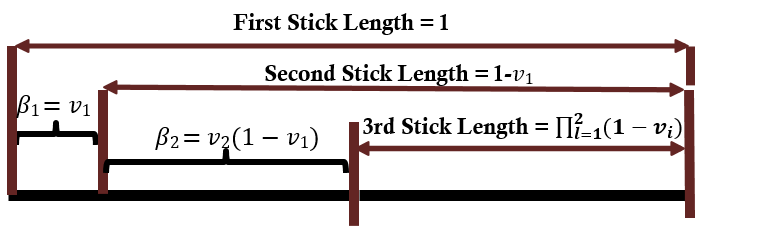
\includegraphics[scale=0.7]{fig13_3.png} 
\caption{Stick-Breaking Construcion}
\label{fig:13-3}
\end{figure}
이를 방지해주면서 sampling을 가능케하는 것이 stick-breaking construction의 핵심이라 할 수 있다. stick-breaking construction은 stick의 전체 길이 (첫 시행에서 stick의 길이는 1로 한다.)를 기준으로 beta distribution에 따라 sampling을 하되, 그 다음 sampling에서는 전 sample의 길이만큼을 제외한 나머지 stick의 길이를 기준으로 sampling하는 방식을 의미한다. 

아래의 식에서 $\beta_{k}$은 전체 스틱의 길이를 1로 정의하였을 때 k번째 sampling시 해당 sample이 차지하는 길이를 의미한다. 여기서 각 sample이 차지하는 길이는 곧 해당 choice가 선택될 확률을 의미한다. 또한 이러한 특성을 만족하는 $\beta$를 Common notation으로 다음과 같이 표기한다. 
\begin{equation}
\beta_{k}=v_{k}\Pi^{k-1}_{l=1}(1-v_{l})\;\;\rightarrow\;\;\beta \sim GEM(\alpha)
\end{equation}
위의 방식을 통해 무한한 choice number k에 대해서도 probability axiom을 만족하면서 sampling이 가능함을 확인하였다. 이제 본 방식을 Dirichlet process에 적용해보면 다음과 같이 나타낼 수 있다.\\

* Stick-Breaking Construction for Dirichlet process
\begin{eqnarray}
G|\alpha,H&\sim&DP(\alpha,H) \\
\beta \sim GEM(\alpha)\;\;,\;\;G &=& \sum^{\infty}_{k=1}\beta_{k}\delta_{\theta_{k}}\;\;,\;\;\theta_{k}|H \sim H
\end{eqnarray}

$\beta \sim GEM(\alpha)$에서 $\alpha$는 Beta distribution의 두 번째 parameter $\beta^{*}$를 의미한다는 것을 확인하였다. (GEM의 $\beta$와 중복되기 때문에 $\beta^{*}$라고 하겠다.) $\beta^{*}$값이 변함에 따라 sampling되는 각각의 $v$값에도 변화가 발생할 것인데, 아래의 그래프가 이를 잘 나타내주고 있다. \\
\begin{figure}[ht] \centering 
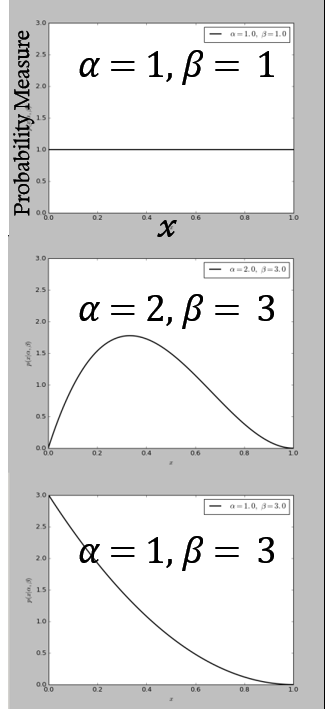
\includegraphics[scale=0.7]{fig13_4.png} 
\caption{$\beta^{*}$값의 변화에 따른 Beta distribution의 변화}
\label{fig:13-4}
\end{figure}

위의 그래프를 통해 $\beta^{*}$의 값이 1일 경우 sampling되는 $v$의 값이 상대적으로 크며 반대로 $\beta^{*}$의 값이 3일 경우 sampling될 $v$의 값이 상대적으로 작아짐을 알 수 있다. 이를 통해 우리는 cluster나 choice 개수 $k$에 대한 각각의 확률을 정하는 단계에서 $\beta^{*}$의 값, 즉 $\alpha$의 값 조정을 통해 확률에 대한 민감도(Sensitivity)를 임의로 정할 수 있음을 알 수 있다. 가령 $\alpha$의 값이 클 경우 각 Choice 혹은 클러스터가 가질 개별 확률은 상대적으로 작아질 것이며 $\alpha$의 값이 작을 경우 각각 큰 값을 가진 Cluster 확률값이 나오게 될 것이다. 이러한 방식으로 각 Cluster를 구성할 경우 cluster이자 Choice의 개수 $k$는 임의로 정의내려주는 값이 아니라 각각의 확률값에 의해 결과적으로 정의되는 값이 될 것임을 유추할 수 있다. 또한 stick-breaking의 방식에 따라 각 클러스터의 확률값은 갈수록 줄어드는 양상을 보일 것이기에 의미있는 값을 가지는 cluster의 개수를 어렵지 않게 찾아낼 수 있을 것이다.



\subsection{Polya Urn scheme}
%-----------------------------------------------------------------
Dirichlet process의 sampling 방식으로 유효하게 쓰일 수 있는 두번째 scheme인 Polya urn scheme에 대해 알아보도록 하겠다.  \\

*Dirichlet process
\begin{equation}
G\;|\;\theta_{1}...\theta_{n},\alpha,H \;\sim\; DP(\alpha+n , \frac{\alpha}{\alpha+n}H+\frac{n}{\alpha+n}\frac{\sum^{n}_{i=1}\delta_{\theta_{i}}}{n})
\end{equation}
위의 Dirichlet process에 대한 식을 통해 이번에는 아래의 값을 나타내는 식을 구해보자.
\begin{equation}
\theta_{n}|\theta_{1}...\theta_{n-1},\alpha,H
\end{equation}
위의 식에서 $\theta$는 각 데이터 instance에 대한 값, $\alpha$는 sensitivity parameter, H는 Base distribution을 의미한다. 즉, 1부터 n-1까지의 data instance에 대한 값이 결정되었을 때 그 다음 data의 값을 나타내는 식인 것이다. 이를 나타내면 아래와 같다.
\begin{equation}
\theta_{n}|\theta_{1}...\theta_{n-1},\alpha,H \sim DP(\alpha+n-1,\frac{\alpha}{\alpha+n-1}H + \frac{n-1}{\alpha+n-1}\frac{\sum^{n-1}_{i=1}\delta_{\theta_{i}}}{n-1})
\end{equation}
또한 위의 식에 대한 expectation을 구해보면 아래와 같다.
\begin{equation}
E[\theta_{n}|\theta_{1}...\theta_{n-1},\alpha,H] \sim \frac{\alpha}{\alpha+n-1}H+\frac{\sum^{n-1}_{i=1}\delta_{\theta_{i}}}{\alpha+n-1}
\end{equation}
위의 식에서 $\sum^{n-1}_{i=1}\delta_{\theta_{i}}$을 조금 더 들여다보자. $\delta_{\theta_{i}}$의 경우 i번째 data가 특정 cluster에 포함되는 지 안되는 지에 따라 0,1의 값을 갖는 변수이다. 고로 $\sum^{n-1}_{i=1}\delta_{\theta_{i}}$은 n번째 data를 제외한 나머지 data에 대한 선택 결과를 나타내는 식이라 볼 수 있다.

이를 각 data에 대한 summation이 아닌 cluster 별 summation에 대한 식으로 나타내면 아래와 같이 쓸 수 있다. 
\begin{equation}
\sum^{n-1}_{i=1}\delta_{\theta_{i}} \rightarrow \sum^{K}_{k=1}N_{k}\delta_{\theta_{k}}
\end{equation}

$\delta_{\theta_{k}}$의 경우 특정 cluster를 정확히 가리킬 때만 1의 값을 가지며 $N_{k}$의 경우 각 클러스터에 속한 데이터의 갯수를 나타내는 변수이다. 위와 같이 변환된 식을 바탕으로 $\theta_{n}|\theta_{1}...\theta_{n-1},\alpha,H$을 나타내면 아래와 같다. 
\begin{equation}
E[\theta_{n}|\theta_{1}...\theta_{n-1},\alpha,H] \sim DP(\alpha+n-1,\frac{\alpha}{\alpha+n-1}H + \frac{n-1}{\alpha+n-1}\frac{\sum^{K}_{k=1}N_{k}\delta_{\theta_{k}}}{n-1})
\end{equation}
결국 Polya Urn Scheme을 통해 우리는 Dirichlet process에서의 임의의 observation을 sampling할 수 있다. 또한 그 과정에서 효율적인 점은 $\theta$를 sampling할 때 이에 대한 distribution인 $G|\alpha,H$를 sampling하지 않아도 된다는 것이다. 이러한 특성은 distribution G를 sampling할 때 유용하게 쓰이는 stick-breaking과는 다소 다른 특성이라 볼 수 있다. Polya urn은 확률 및 통계에서 자주 언급되는 우화이기도 하다. 어떤 의미를 갖는 우화인지에 대해 알아보고 가도록 하겠다. \\

* Polya Urn Scheme

1) Create an empty urn

2) Do
\begin{eqnarray}
\;\;\;\;\;\;toss & = & Coin\; toss\; from\; |0,\alpha+n-1|\nonumber\\
\;\;\;\;\;\;if\;\; 0 &\leq& toss < \alpha \rightarrow Add\;a\; ball\; to \;the\; urn\; by\; painting \;the\; ball\; as\; a\;sample\;from\;\theta_{n}\;\sim \;H\nonumber\\
\;\;\;\;\;\;if\;\; \alpha &\leq& toss < \alpha + n -1 \rightarrow pick\; a \;ball\; from\; the\; urn \;and \;return\; the\; ball\; and\nonumber\\
&  & a\; new\; ball\; with\; the\; same\; color\; to\; the\; \nonumber
\end{eqnarray}
위의 우화는 결국 Coin toss 결과에 따라 다른 행위를 정의하고 있는데, 먼저 Coin toss 결과가 $\alpha$보다 작을 경우 새로운 ball을 넣어준다. 다만 그 ball의 색깔을 결정하는 것은 base distribution인 H가 되는 것이다. 예를 들어 n=1일 경우 $\alpha +n-1$은 무조건 0과 $\alpha$사이의 값을 가지므로 처음에는 무조건 새로운 ball 하나를 넣어줘야할 것이다. 

그 다음 횟수부터 만약 Coin toss가  $\alpha$ 이상 $\alpha+n-1$이하의 값을 가질경우 우리는 현재 urn안에 넣어진 공 중 하나를 추출하여 그 공과 같은 색의 공을 하나 추가해줄 것이다. 이러한 iteration이 지속적으로 반복될 경우 n이 커질수록 urn에 많이 담긴 색의 공이 갈수록 더 많아지는 이른바 '부익부 빈익빈' 현상이 발생할 것이다. 

\begin{figure}[ht] \centering 
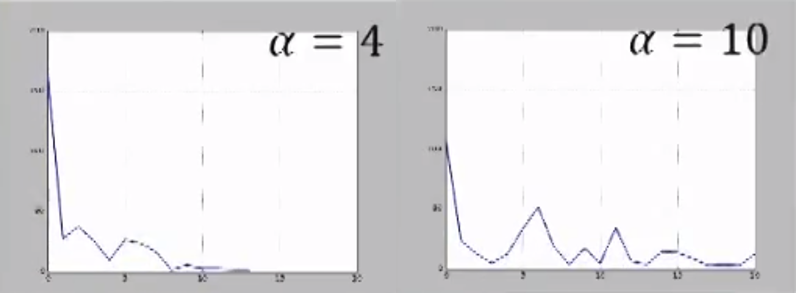
\includegraphics[scale=0.7]{fig13_5.png} 
\caption{$\alpha$값의 변화에 따른 Cluster index(ball)별 개수}
\label{fig:13-5}
\end{figure}

그렇다면 Polya Urn scheme의 방식에 영향을 주는 $\alpha$의 값에 따라 그 결과가 어떻게 변할까? 이는 위의 식을 통해 어렵지 않게 유추할 수 있다. 만약 $\alpha$값이 크다면 n이 커짐에 상관없이 상대적으로 새로운 ball을 sampling할 가능성이 높아질 것이고 이에 따라 ball별 부익부 빈익빈 현상은 상대적으로 완화될 것이다. 허나 $\alpha$의 값이 상대적으로 작다면 처음에 자주 추출된 ball이 계속해서 추출되어 거대 cluster가 되는 이른바 '부익부빈익빈' 현상이 심화되는 경향이 나타날 것이다. 이러한 경향성을 위의 그림을 통해 알 수 있다. 

\subsection{Chinese restaurant scheme}
%-----------------------------------------------------------------
마지막 Generation scheme으로 Chinese restaurant scheme에 대해 알아보겠다. Chinese restaurant scheme의 경우 polya urn scheme과 크게 다르지 않은 sampling 방식인데, 즉 stick breaking scheme의 주 목적인 distribution construction이 아닌 각각의 data-instance에 대한 sampling이 주 목적이라 할 수 있다. 
\begin{equation}
E[\theta_{n}|\theta_{1}...\theta_{n-1},\alpha,H] \sim DP(\alpha+n-1,\frac{\alpha}{\alpha+n-1}H + \frac{n-1}{\alpha+n-1}\frac{\sum^{K}_{k=1}N_{k}\delta_{\theta_{k}}}{n-1})
\end{equation}
위의 식은 Polya urn scheme에서도 볼 수 있었던 식이다. 결국 Chinese restaurant scheme과 Polya urn scheme은 같은 방식을 통해 sampling을 해나간다는 것을 알 수 있다. $\alpha$의 경우 각각의 Cluster를 얼마나 크게 하며 weight를 어느정도 줄 지 결정하는 parameter이며 $N_{k}$의 경우 k번째 cluster에 assign을 받은 data instance의 개수를 의미한다. 
\begin{equation}
P(\theta_{n}|\theta_{1}...\theta_{n-1},\alpha) = 
\begin{cases} 
\frac{N_{k}}{\alpha+n-1}\\
\frac{\alpha}{\alpha+n-1}
\end{cases}
\end{equation}
결국 위의 식은 n번째 data instance가 어떠한 cluster를 형성할 지를 결정하는 식이라 할 수 있는데, 가령 $\frac{N_{k}}{\alpha+n-1}$의 경우 이미 만들어진 cluster 중 k번째 cluster에 assign될 확률을 나타내며 $\frac{\alpha}{\alpha+n-1}$의 경우 새로운 cluster를 만들어낼 확률이라 칭할 수 있다. 

Polya urn scheme이 ball과 색깔의 metaphor를 이용해 scheme을 설명하였다면 chinese restaurant는 같은 개념을 table에 비유하여 설명하고자 한다. 이에 대해 graphical하게 표현하면 다음과 같이 나타낼 수 있다. \\
\begin{figure}[ht] \centering 
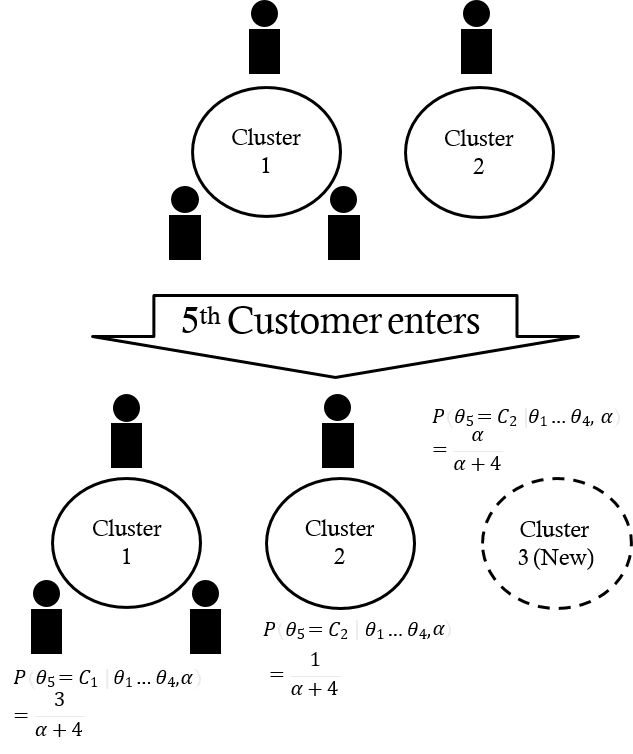
\includegraphics[scale=0.7]{fig13_6.png} 
\caption{Chinese restaurant scheme}
\label{fig:13-6}
\end{figure}
위의 그림은 다섯번째 손님이 table에 앉게 되는 상황에 대해 표현해주고 있다.

직관적으로 알 수 있다시피 첫번째 손님은 다른 선택의 여지없이 첫번째 table에 무조건 착석하게 되고 그 다음 손님부터는 위의 식과 같은 확률로 이미 만들어진 table에 앉게 되거나 (첫 table은 $\frac{3}{\alpha+n-1}$, 두번째 table은 $\frac{1}{\alpha+n-1}$) 혹은 새로운 table에 혼자서 착석하게 될 것이다. ($\frac{\alpha}{\alpha+n-1}$) 

이러한 Chinese restaurant scheme의 작동 방식과 특성을 정리하면 아래와 같다.\\

* Chinese restaurant process

1) Assume infinite number of tables in a restaurant

2) First customer sits at the first table

3) Loop for Customer N sits at
\begin{eqnarray}
&\rightarrow& table\; k\; with\; P(\theta_{n}|\theta_{1}...\theta_{n-1},\alpha) = \frac{N_{k}}{\alpha+n-1}\nonumber\\
&\rightarrow& A\; new \;table\; k+1\; with \; P(\theta_{n}|\theta_{1}...\theta_{n-1},\alpha) = \frac{\alpha}{\alpha+n-1}\nonumber
\end{eqnarray}

* Properties of Chinese

1) Clustering formation

2) Rich-get-richer property

3) No fixed number of clusters with a fixed number of instances

4) Almost identical to Polya Urn Scheme

\subsection{Detour : Random Process}
%-----------------------------------------------------------------
이번 장에서는 Random process에 대해 다시 한번 이야기해보겠다. Gaussian process가 대표적인 Random prcess이며 이번 단원의 주제인 Dirichlet distribution 또한 Random process 중 하나이다. \\

* Random process a.k.a stochastic process 
\begin{center}
    An infinite indexed collection of random variables, $\{X(t)|t \in T\}$\\
    index parameter : t (Can be time, space...)
\end{center}
위의 식이 가지는 정의를 참고했을 때, 결국 무한한 갯수의 cluster를 가정하여 차례대로 만들어나가는 dirichlet process 또한 위의 정의와 일맥상통함을 알 수 있다. 위의 정의를 통해 Random process의 function을 아래와 같이 정의할 수 있다.\\

* A function $X(t,w)$, where t $\in$ T and $\omega$ $\in$ $\Omega$
\begin{center}
    Outcome of the underlying random experiment : $\omega$\\
    Fixed t $\rightarrow$ X(t,$\omega$) is a random variable over $\Omega$\\
    Fixed $\omega$ $\rightarrow$ X(t,$\omega$) is a deterministic function of t, a sample function
\end{center}
위와 같이 t와 $\omega$로 나타내어진 function X(t,$\omega$)에서 만약 t를 고정시켜 특정 time에 대한 값을 본다면 이는 해당 t의 시점에 sampling된 output에 대한 분포를 나타내어줄 것이다. 또한, 다른 변수인 $\omega$를 고정시킨다면 이는 t에 의한 함수인 time-series function이 될 것이며  이는 각각의 iteration마다의 output에 대한 trajectory (경로)의 형태로 결과가 나올 것임을 짐작할 수 있다. 

\begin{figure}[ht] \centering 
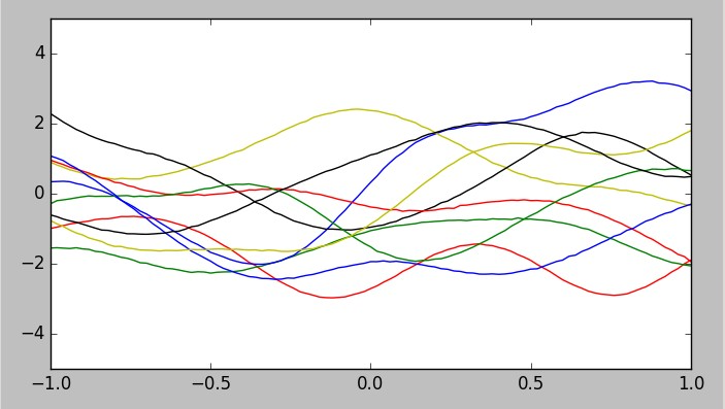
\includegraphics[scale=0.5]{fig13_7.png} 
\caption{변수 t의 변화에 따른 각 sample 별 X(t,$\omega$) 변화 추이}
\label{fig:13-7}
\end{figure}

\subsection{de Finetti's Theorem}
%-----------------------------------------------------------------
앞의 장을 통해 Dirichlet process 또한 Random process (a.k.a stochastic process)의 한 종류임을 알게 되었다. 이번에는 dirichlet process이 가진 Random process의 특성을 더 numerical하게 해석하기 위해 de Finetti's theorem에 대해 논해보도록 하겠다. de Finetti's theorem에 대한 이해를 위해 먼저 Exchangeability에 대해 알아보자.\\

* Exchangeability

A joint probability distribution is exchangeable if it is invariant to permutation (Given a permutation of $S$)
\begin{eqnarray*}
    P(x_{1},x_{2},...,x_{N}) = P(x_{S_{1}},x_{S_{2}},...,x_{S_{N}})
\end{eqnarray*}
Permutation에 invariant하다는 것은 결국 위와 같이 각 instance의 순서가 뒤바뀌어도 전혀 영향을 받지 않는다는 것이며 결국 이를 만족하는 joint probability distribution이 exchangeable하다고 말할 수 있는 것이다. 이를 활용하여 De Finetti theorem을 정의하면 아래와 같다.\\

* (De Finetti, 1935) 
\begin{center}
If $(x_{1},x_{2},...)$ are infinitely exchangeable, then the joint probablity $P(x_{1},x_{2},...,x_{N})$ has a representation as a mixture
\begin{equation}
P(x_{1},x_{2},...,x_{N}) = \int(\Pi^{N}_{i=1}P(x_{i}|\theta))dP(\theta) = \int P(\theta)(\Pi^{N}_{i=1}P(x_{i}|\theta))d\theta
\end{equation}
\end{center}
결국 특정 joint probability distribution을 prior의 형태인 $P(\theta)$와 likelihood의 형태인 $\Pi^{N}_{i=1}P(x_{i}|\theta)$로 표현할 수 있는 것이다.\\
더 나아가 exchangeability와 IID (independent and identically distributed) 사이의 관계에 대해 이야기해보자. 가령 IID의 대표적인 예시인 동전 던지기의 경우 각각의 시행에 대한 교환을 하는 것이 전혀 확률에 영향을 주지 않는다. 고로 IID일 경우 exchangeable하다고 이야기할 수 있다.\\
그렇다면 exchangeable할 경우 IID (independent and identically distributed)이라고 말할 수 있는가? 그렇지 않다. Polya urn sampling이 이를 설명하는 가장 좋은 예시인데, Polya urn sampling은 IID의 특성을 가지지 않는다. 이전의 시행에 대한 결과로 나타난 공의 분포가 그 다음 뽑힐 공에 대한 확률에 영향을 미치기 때문이다. 하지만 Polya urn sampling을 infinite하게 시행한다고 가정하면, 결국 가능한 모든 cluster가 출현하게 될 것이다. 이 경우 각각의 sampling에 대한 출현 순서를 바꾸더라도 결과적인 확률값에 영향을 주지 않을 것임을 유추할 수 있다. 
\begin{equation}
For\; some\; ramdom\; variable\; \theta\;
\begin{cases} 
independent\; and\; identically\; distributed \rightarrow Exchangeable\; : \;Yes \\
Exchangeable \rightarrow IID\; :\; No.\; counter \;example\;is \;Polya\; urn \;sampling
\end{cases}
\end{equation}
그렇다면 이러한 특성이 시사하는 바는 무엇일까?  Polya urn scheme이 exchangeable함을 보인 것 처럼 같은 방식으로 sampling을 진행하는 Chinese restaurant process 또한 exchangeable하다는 결론을 내릴 수 있는데, 이는 Gibbs sampling의 간단한 derivation에 매우 효과적인 기법이 될 수 있다.\\
만약 exchangeablity를 모델에 적용할 수 있다면 i번째 data instance에 대한 cluster assignment를 할 때 그 순서에 구애받지 않고 assignment가 가능해질 것이다. 예를 들어, 총 n개의 data instance에 대해 일시적인 cluster assignment를 한 후 i번째 data instance의 cluster assignment를 나머지 n-1개의 data에 대한 cluster 분포를 통해 다시 결정지으며 그 다음에는 나머지 data instance들 중 하나를 골라 같은 방식으로 assignment를 해줄 수 있다. 이를 통해 Gibbs sampling에 대한 방법론의 수학적인 증명이 가능함을 보일 수 있다.

\section{Dirichlet process Mixture Model}
%-----------------------------------------------------------------
지금까지 Dirichlet process의 정의 및 특성과 함께 distribution의 Construction방식, data-instance의 sampling 방식에 대해 알아보았다. 이를 바탕으로 dirichlet process를 Gaussian mixture model에 적용한 예시인 Dirichlet process mixture model에 대해 알아보도록 하겠다.
\subsection{Detour : Gaussian Mixture Model}
%-----------------------------------------------------------------
Gaussian Mixture model은 multiple multivariate Gaussian distribution이 mixture 되었을 때의 model, 즉 여러 개의 gaussian distribution이 융합(mixture)되어 하나의 distribution을 이룰 때 쓰이는 model이다. 이를 수식으로 나타내면 다음과 같이 표현할 수 있다.
\begin{equation}
P(x) = \sum^{K}_{k=1}P(z_{k})P(x|z) = \sum^{K}_{k=1}\pi_{k}N(x|\mu_{k},\Sigma_{k})
\end{equation}
위의 식에서 k에 대한 각각의 $\pi_{k}$는 각각의 distribution을 어떤 비율로 linear하게 합쳐줄지를 나타내는 mixing coefficient이며 $(x|\mu_{k},\sum_{k})$은 k개로 나누어진 각각의 distribution을 나타내는 component이다. 결국 k를 통해 우리는 component 갯수를 결정할 수 있으며 이를 자유롭게 제어할 수 있도록 하기 위해 dirichlet process가 필요한 것이다. 

결국 parameter $\pi$의 dimension인 k는 GMM에 mixture된 distribution의 개수를 의미하며 이 숫자 k가 결국 변수 z와 parameter $\mu$와 $\sum$에 까지 영향을 주는 구조임을 알 수 있다. 

이러한 k를 자유롭게 제어해주기 위해서는 크게 2가지가 필요하다. 첫번째, $\pi$를 bayesian 형태로 바꾸어 k를 조정할 수 있게끔 해야하며 두번째, sampling distribution이 무한대로 가는 상황에서도 유효하게 작동할 수 있도록 non-parametric한 특성을 반영해주어야 한다.

\subsection{Dirichlet process mixture model}
%-----------------------------------------------------------------
이제 본격적으로 DPMM (Dirichlet Process Mixture model)에 대해 알아보겠다. $\pi_{k}$는 항상 multinomial distribution의 k-th choice에 대한 확률로 쓰였으며 multinomial distribution을 z에 대해 나타내면 아래와 같이 나타낼 수 있었다.
\begin{equation}
z_{k} \in ({0,1}), \;\sum_{k}z_{k}=1,\; P(z_{k}=1)=\pi_{k}\;,\sum^{K}_{k=1}\pi_{k}=1,\; 0\leq \pi_{k} \leq 1
\end{equation}

이러한 특징에 큰 영향을 주는 k에 대한 자유로운 제어를 위해서는 먼저 Model의 $\pi$에 해당하는 부분을 baysian 형태로 나타내주어야 한다. 아래의 figure에서 indicator view graphical model이 이를 잘 표현해주고 있는데, 종래에 $\pi$가 있던 부분이 없어지고 $\beta$가 들어왔으며 $\beta$에 영향을 주는 hyper-parameter $\gamma$가 새롭게 등장했음을 알 수 있다.

k에 대한 제어를 위해서는 baysian 형태로 바뀐 모델에 무한대의 k에 대한 적용이 가능토록 non-parametric의 특성 또한 부여해주어야 한다. 이러한 필요성 또한 $\theta$와 이에 영향을 주는 $\lambda$로 잘 소개되어있다. ($\lambda$또한 baysian의 특성을 위해 반영된 hyper-parameter라 할 수 있다.) 여기서 주의할 점은 결국 $\theta$의 $\infty$ 표현이 유효하려면 $\beta$또한 무한대로서 표현을 해주어야한다는 사실이다. 앞의 GMM 모델을 통해 cluster 개수를 나타내는 $\pi$와 centroid 개수를 나타내는 $\mu$,$\sum$은 서로 같은 dimension을 갖는다는 것을 이미 잘 알고있다.

graphical model의 특성을 반영한 infinite k값을 가진 GMM을 나타내면 아래와 같다.\\
* Indicator representation of GMM with infinite K
\begin{center}
$\beta|\gamma \sim GEM(\gamma), \; \theta_{k}|H,\lambda \sim H(\lambda),\;z_{i}|\beta \sim \beta,\;x_{i}|{\theta_{k}}^{\infty}_{k=1},z_{i} \sim F(\theta_{z_{i}})$\\
$\beta \sim GEM(\alpha) \rightarrow k=1,2,...,\infty, v_{k}|\alpha \sim Beta(1,\alpha), \beta_{k} = v_{k}\Pi^{k-1}_{l=1}(1-v_{l})$
\end{center}
위의 GEM distribution은 stick breaking scheme에서 쓰였던 distribution이다. 위에서 배웠다시피 stick breaking scheme은 infinite한 distribution construction이 필요할 때 쓰이는 기법이다. 결국 GEM distribution을 통해 sample되는 각각의 $\beta$에 대한 dimension은 자연스럽게 무한대($\infty$)로 발산하게 될 것이다.

또한, $\theta$의 경우 $\lambda$에 의해 영향을 받는 base distribution H라고 가정할 수 있으며 $z_{i}$의 경우 $\beta$의 각 dimension에 대한 확률값으로 인해 multinomial distribution의 형태로 영향을 받을 것이다. 마지막으로 data $x_{i}$의 경우 특정 클러스터가 지정되었을 때 이에 해당하는 $\theta_{z_{i}}$에 의해 결정된 distribution의 확률값에 영향을 받게 될 것이다. 이를 모두 종합한  indicator view graphical model을 보면 특성들이 잘 반영되어 있음을 알 수 있다. graphical model을 확인하는 과정에서 $\theta$에 대한 궁금증이 발생할 수 있는데, $\theta$는 쓰이는 distribution의 parameter에 따라 그 형태를 달리한다. 가령, distribution의 종류로 Gaussian distribution을 쓰게 된다면 $\theta$는 $\mu$와 $\sigma$의 형태로 표현할 수 있다.
\begin{figure}[ht] \centering 
\begin{center}
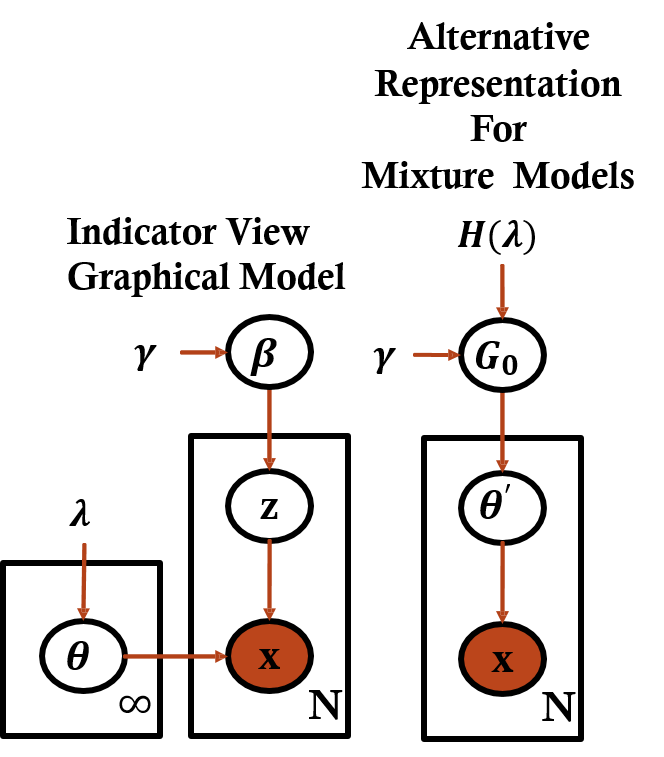
\includegraphics[scale=0.6]{fig13_8.png} 
\caption{DPMM의 두가지 모델 표현 방식 (indicator view graphical model (좌), alternative representation model (우))}
\label{fig:13-8}
\end{center}
\end{figure}

다음으로 indicator view Graphical model을 다른 방식으로 나타낸 Alternative Representation model(For Mixture models)에 대해 살펴보자. 실제로 Mixture model과 관련된 논문들에선 alternative representation으로 표현된 모델을 훨씬 자주 볼 수 있다.

실제로 아래의 그림을 비교하면 알 수 있다시피 $\beta$가 들어갔던 자리에 DP를 따르는 $G_{0}$가 새로이 자리잡아 있으며 Z가 들어가던 자리에 $\theta^{'}$가 있음을 알 수 있다. 

이를 바탕으로 infinite K에 대한 GMM의 alternative representation을 아래와 같이 정의하도록 한다.

* Alternative representation of GMM with infinite K
\begin{center}
$G_{0}|H,\gamma \sim DP(\gamma,H), \theta^{'}_{i}|G_{0} \sim G_{0}, X_{I}|\theta^{'}_{i} \sim F(\theta^{'}_{i})$\\
$\theta_{n}|\theta_{1}...\theta_{n-1},\gamma,H \sim DP(\gamma+n-1,\frac{\gamma}{\gamma+n-1}H + \frac{n-1}{\gamma+n-1}\frac{\sum^{K}_{k=1}N_{k}\delta_{\theta_{k}}}{n-1})$
\end{center}
위의 식에서 $\theta^{'}$는 분명 indicator representation에서의 $\theta$ 와는 다른 의미를 지니고 있다. Chinese restaurant scheme을 예로 들어 생각해보자. 각각의 사람들이 배치받는 table을 $\theta$ 라고 표현하였고 이에 대해 각각의 사람에 대한 assignment를 담당하는 것이 z였다면, alternative representation에서는 z와 $\theta$가 함께 나타낸 부분을 $\theta^{'}$ 하나로 표현하고자 한다. 

즉 $\theta^{'}_{i}$는 각각의 data가 각 table에 배치되는지에 대한 여부를 0 또는 1로 나타내는 index 형태로 존재하는 것이다. 각각의 $\theta^{'}_{i}$는 특정 table (cluster)에 잠정적으로 배치되어 있을 것이며 각각의 table에 $\theta^{'}_{i}$이 배치된 결과를 수식화한 likelihood를 바탕으로 모델 각각의 parameter를 update할 수 있을 것이다. 

위를 통해 우리는 indicator view와 alternative representation의 근본적 차이점을 알아낼 수 있다. indicator view는 GEM, 즉 stick breaking construction과 같은 방식을 통해 $\beta$에 대한 distribution을 명시적으로 표현해주었다면 Alternative representation의 경우는 각각의 data instance에 대한 sampling process에 초점을 맞춘 방식이라 할 수 있다. 

우리는 GMM에 대하여 Alternative representation 방식을 사용하며 설명을 해나가고자 한다. 즉, 각각의 instance을 sampling할 때 마다 이전의 assignment 상태를 고려하여 해당 instance를 assign해주며 이에 따라 parameter를 update해주는 것이다. 

허나 각각의 $\theta^{'}_{i}$에 assign된 cluster(choice)는 parameter의 update 과정에서 달라질 가능성이 있다. DPMM의 모태인 Dirichlet process는 반드시 de Finetti's theorem 를 만족해야 하기 때문이다. 이를 통해 $\theta^{'}_{i}$ 각각이 지정된 cluster에 대한 likelihood 비교를 통해 parameter를 update해줌은 물론 $\theta^{'}_{i}$의 각 cluster별 확률값 또한 지속적으로 바뀌게 된다. 


\subsection{Implementation Details of DPMM}
%----------------------------------------------------------------
DPMM에서는 Component parameter를 Online update하는 방식으로 모델을 학습시킨다. 이에 대한 예시를 더 구체적으로 들어보자.
\begin{center}
$G_{0}|H,\gamma \sim DP(\gamma,H), \theta^{'}_{i}|G_{0} \sim G_{0}, X_{I}|\theta^{'}_{i} \sim F(\theta^{'}_{i})$\\
$\theta_{n}|\theta_{1}...\theta_{n-1},\gamma,H \sim DP(\gamma+n-1,\frac{\gamma}{\gamma+n-1}H + \frac{n-1}{\gamma+n-1}\frac{\sum^{n-1}_{i=1}\delta_{\theta_{i}}}{n-1})$
\end{center}
Gaussian mixture model에 대해 각각의 cluster (table)이 가지는 parameter를 $\mu_{i}$와 $\sum_{i}$라고 해보자. 첫번째 table에 $\theta^{'}_{1}$과 $\theta^{'}_{2}$, $\theta^{'}_{3}$가 앉아있고 두번째 table에 $\theta^{'}_{4}$이 앉아있는 상황이라면, $\theta^{'}_{5}$이 첫번째 table에 앉을 확률은 $\frac{\sum^{4}_{i=1}\delta_{\theta_{1}}}{\gamma+n-1}$, 두번째 table에 앉을 확률을 $\frac{\sum^{4}_{i=1}\delta_{\theta_{2}}}{\gamma+n-1}$, 새로운 table에 앉을 확률을 $\frac{\gamma}{\gamma+n-1}$이라 칭할 수 있다. 전에 비교하여 달라진 부분은 바로 특정화되지 않은 F function을 gaussian의 형태로 하는 것이다. 
\begin{equation}
F(x_{i}|\theta^{'}_{i})=N(x_{i}|\mu_{\theta^{'}_{i}},\Sigma_{\theta^{'}_{i}})
\end{equation}
$\mu_{\theta^{'}_{i}}$의 형태를 볼 수 있듯이 각각의 $\mu$와 $\sum$에 각 $\theta$의 table assignment에 대한 정보가 포함되어 있음을 알 수 있다. 이를 통해 각각의 cluster (table)에 대한 parameter의 계산은 해당 cluster (table)에 assign된 data point를 통해 수행할 수 있을 것이며 이를 통해 update 또한 가능해질 것이다. DPMM을 수행하는 일련의 과정을 psuedo code 형태로 나열하면 아래와 같이 나타낼 수 있다.\\

* DPMM\\
 initial table assignments\\
 While sampling iteration\\
 While each data instance in the dataset
 \begin{center}
  1) Remove the instance from the assignment\\
  2) Calculate the prior : $\theta_{n}|\theta_{1},...,\theta_{n-1},\gamma,H \sim DP$\\
  3) Calculate the likelihood : $N(x_{i}|\mu_{\theta^{'}_{i}},\sum_{\theta^{'}_{i}})$\\
  4) Calculate the posterior\\
  5) Sample the cluster assignment from the posterior\\
  6) Update the component parameter\\
  \end{center}
처음에는 총 N개의 data instance에 대한 table assignment가 필요할 것이다. 그 다음 각각의 data instance에 대한 sampling process가 진행되는데, 이 과정에서 de Finetti theorem이 효력을 발휘한다.

즉, 각각의 data instance에 assignment가 완료된 상황에서 i의 순서에 관련없이 각 $\theta^{'}_{i}$에 대한 sampling을 다시 수행하는 것이다. 만약 n개의 data가 존재한다면 해당 i번째 data를 제외한 나머지 n-1개의 data에 대한 assignment 정보를 통해 $\theta^{'}_{i}$의 prior 값을 결정하게 될 것이다. 그 후에는 i번째 data instance가 각각의 table(cluster)에 앉을 경우에 대한 likelihood를 계산해주어야 한다. 

여기서 의문이 들 수 있는 부분은 새로운 cluster (table)에 대한 likelihood는 어떻게 정의하냐는 점이다. 아직 data가 assign되지 않은 경우 parameter ($\mu$, $\sum$)에 대한 계산도 어렵고, 때문에 likelihood에 대한 계산도 불가능하리라 여기기 쉽기 때문이다. 이를 가능케 해주는 것이 바로 Base distribution H이다. 즉, Base distribution에서 임의로 뽑아낸 parameter $\mu$, $\sum$의 값을 새로운 cluster (table)에 이용하는 것이다. 

이를 통해 prior와 likelihood를 구한 후에는 마침내 Posterior distribution를 구할 수 있게 된다. 구한 Posterior distribution을 바탕으로 cluster assignment를 실행하며 이를 통해 component parameter를 학습시키는 과정을 거친다. 

이러한 전체 과정을 이해한다면  data (likelihood)가 cluster assignment에 영향을 미치는 부분과 prior가 영향을 미치는 부분에 대한 명확한 구분 또한 가능할 것이다.

먼저 likelihood의 경우 각 data가 임의의 cluster에 뭉침으로써 likelihood가 커지는 양상을 보인다면 실제 assignment에서도 해당 data를 서로 같은 cluster에 assign되게끔 영향을 줄 것이다. 그 다음, prior의 경우 각 table에 배정된 data의 갯수를 비교하며 상대적으로 큰 cluster에 data가 더욱 쏠리게 하는 이른바 '부익부 빈익빈' 현상에 일조할 것이다. 결국 이 두가지 영향을 통해 각각의 cluster가 만들어지는 것이다. 

뿐만 아니라, prior를 통해 DPMM은 무한한 cluster(table)을 만들어낼 수 있는 방식을 제안하였다. 이는 choice 개수인 k에 의해 제한받지 않는 방식임을 이해할 수 있다. 

이를 통해 무한한 cluster k를 만들어낼 경우 생겨날 수 있는 문제는 모델에 큰 영향을 줄 수 없는 cluster (ex : data가 1개 assign되어있는 cluster)가 함께 무한히 생겨날 수 있다는 점이다. 
이를 방지하기 위해 DPMM을 실제로 적용할 때에는 무한한 cluster가 아닌 cluster 개수에 upper limit를 설정하는 방식으로 모델을 만들기도 한다. 이를 Truncated Dirichlet process mixture model이라고 부른다. 


\newpage
\subsection{DPMM Sampling Process}
%-----------------------------------------------------------------
이번 장에서는 DPMM의 Sampling process에 대해 더 자세히 알아보도록 하겠다. 아래의 식은 $\theta^{n}$에 대한 sampling을 나타내는 식으로서, 본래 cluster 개수를 의미했던 k의 역할을  $\gamma$가 수행하고 있음을 알 수 있다.
\begin{center}
$\theta_{n}|\theta_{1}...\theta_{n-1},\gamma,H \sim DP(\gamma+n-1,\frac{\gamma}{\gamma+n-1}H + \frac{n-1}{\gamma+n-1}\frac{\sum^{K}_{k=1}N_{k}\delta_{\theta_{k}}}{n-1})$
\end{center}

\begin{figure}[ht] \centering 
\begin{center}
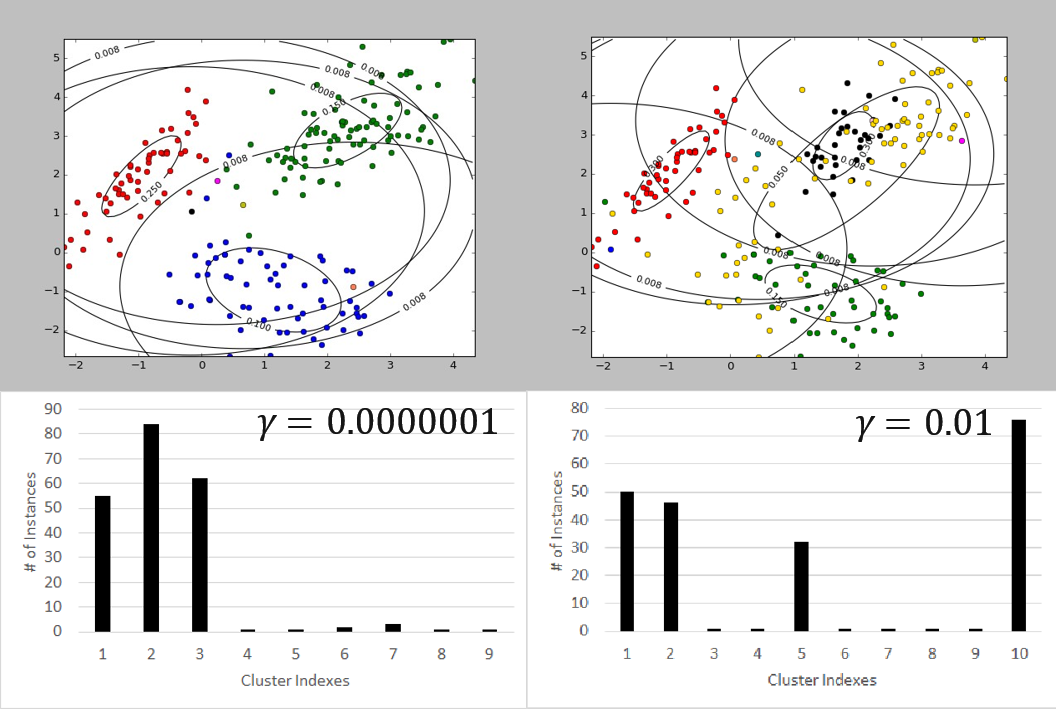
\includegraphics[scale=0.6]{fig13_10.png} 
\caption{$\gamma$의 변화에 따른 synthesized True Dataset에 대한 sampling 결과 변화}
\label{fig:13-9}
\end{center}
\end{figure}


위의 그림에서 $\gamma$의 값이 0.0000001일 경우를 먼저 살펴보면 약 3개의 main cluster가 각각 큰 범위로 자리잡아 있는 것을 알 수 있다. 허나, 그 사이에 몇몇 점의 경우 매우 작은 cluster를 형성하는 data들이 자리잡고 있으며 이는 chinese restaurant scheme에서 다뤘던 새로운 table에 대한 의미를 가지고 있다고 볼 수 있다. 

이번엔 $\gamma$가 0.01인 경우를 살펴보자. $\gamma$의 값이 달라지면서 main cluster라고 할 수 있는 것들의 개수가 4개로 증가하였다. 또한 그 사이에 몇몇 점이 마찬가지로 작은 cluster를 형성하고 있음을 관찰할 수 있다. 눈여겨볼 점은 2개의 main cluster가 서로 중첩된 상황에서 형성되었다는 것이다. 즉, cluster를 약간 벗어난 몇몇 점에 대한 분포를 통해 2개의 distribution이 mixture되어있다고 인식한 것이다. 여기에서 $\gamma$가 가지는 역할을 유추할 수 있다.

$\gamma$가 커질수록 $\frac{\gamma}{\gamma+n-1}H$의 값이 커지며 이는 chinese restaurant scheme에서 의미하는 새로운 table, 즉 새로운 cluster를 생성할 확률이 커지는 것이다. 고로 $\gamma$의 값이 작으면 모델은 반드시 필요한 cluster만을 주요하게 만들어내며 $\gamma$가 커질수록 발견해내지 못한 새로운 cluster를 정의내릴 확률이 높아진다고 이야기할 수 있다. 이로써 k의 값은 정해진 값이 아닌 sensitivity 변수 $\gamma$에 의해 결정되는 추상적인 값이 되며 이를 통해 모델을 nonparametric하게 변화시킴을 확인할 수 있다. 


\section{Hierarchical Dirichlet Process}
%-----------------------------------------------------------------
위의 장을 통해 data가 k의 값을 결정하게끔 도와주는 Dirichlet process를 Gaussian mixture model에 적용한 예시인 DPMM (dirichlet process mixture model)에 대해 알아보았다. Gaussian mixture model이 아닌 다른 cluster model 또한 이러한 k의 제어가 필요하다. 이번 장에서는 이를 가능케 하기 위해 dirichlet process에 계층을 만든 구조인 Hierarchical Dirichlet process에 대해 알아보도록 하겠다. 

\subsection{Problem of Separate Prior}
%-----------------------------------------------------------------
먼저 Hierarchical dirichlet process가 왜 필요한 지에 대해 알아보도록 하겠다.아래의 예시를 살펴보자. 
\begin{figure}[ht] \centering 
\begin{center}
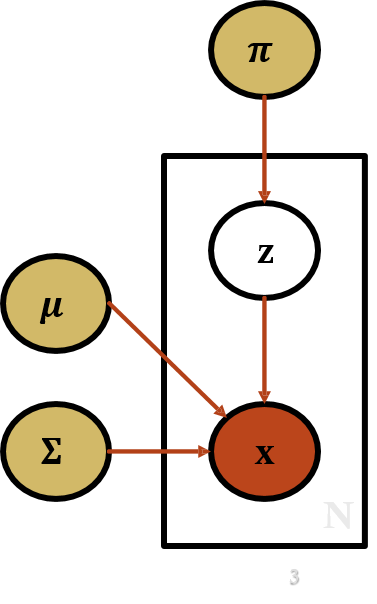
\includegraphics[scale=0.6]{fig13_1.png} 
\caption{graphic model of gaussian mixture model}
\label{fig:13-10}
\end{center}
\end{figure}
rough한 상태의 GMM은 prior에 대한 제어도 불가능하며 data instance에 대한 연관성과 structure가 존재하지 않음을 알 수 있다. 그 다음은 LDA 모델에 대해 살펴보자. 
\begin{figure}[ht] \centering 
\begin{center}
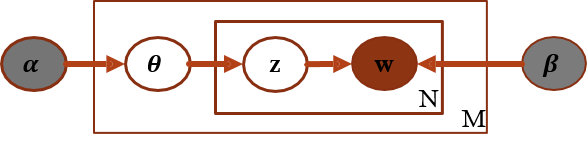
\includegraphics[scale=0.6]{fig13_2.png} 
\caption{graphic model of LDA}
\label{fig:13-11}
\end{center}
\end{figure}
LDA는 임의의 Text corpus를 기반으로 soft clustering을 하는 모델로 잘 알려져있다. 이를 성공적으로 수행하기 위해 corpus에 대한 structure를 정의하고 있는데,  전체 set에서 나오는 모든 word (w)들을 각각의 document에 등장하는 단어로 구조화 (structure)함으로서 Corpus-Document structure를 구성해놓았다. 즉, GMM과는 달리 LDA는 각 데이터에 대한 관계성을 정의할 수 있으며 word, document, corpus로 이어지는 계층적 구조(Hierarchical structure)를 띄고 있음을 알 수 있다. 

이렇듯 k가 finite한 숫자로 정의된 경우에서 Hierarchical structure를 이용한 LDA의 방식은 매우 성공적으로 수행되고 있다. 이를 더 자세하게 나타낸 아래의 그림을 보자. 
\begin{figure}[ht] \centering a
\begin{center}
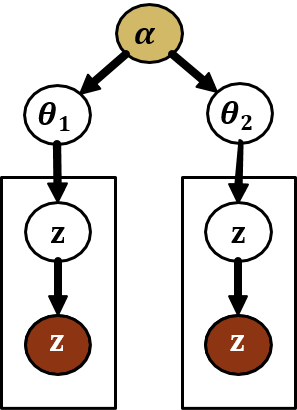
\includegraphics[scale=0.6]{fig13_11.png} 
\caption{detailed graphic model of LDA}
\label{fig:13-12}
\end{center}
\end{figure}
하나의 $\alpha$값에 의해 sampling 된 $\theta_{1}$과 $\theta_{2}$가 각각 [0.1,0.2,0.7], [0.4,0.3,0.3]의 값을 가짐을 알 수 있다. 각각의 dimension에 대한 값은 topic 별 할당 확률을 의미하는데, 당연하게도 $\theta_{1}$과 $\theta_{2}$은 서로 같은 topic dimension을 가질 것이다. 만약 각각의 Choice를 atom으로 비유한다면 위와 같은 상황은 각각의 atom이 잘 overlap된 상황이라 볼 수 있다. 이처럼 Choice의 개수가 finite한 경우 Hierarchical strucuture에서도 atom간의 overlap은 쉽게 만들어낼 수 있다.  

허나 choice k의 개수가 finite하지 않고 infinite한 경우 Atom(Choice)간의 overlap은 잘 만들어지지 않는다. DPMM을 예로 들어 설명해보겠다. DPMM에서 각각의 Choice는 base distribution H에 의해 sampling된 결과로 볼 수 있었다. 허나 continuous한 base distribution에서 임의로 sampling한 특정 값이 언젠가 똑같은 값으로 sampling될 확률은 현저하게 낮다. 이로 인해 atom의 non-overlap 문제가 생겨나며 이를 꼭 해결해주어야 하는 것이다. 

위의 상황을 조금 더 풀어 설명하면, Hierarchical한 구조상에서 choice가 infinite할 때 여러 개의  branch를 만들 경우 각 branch별로 가지는 cluster의 수와 특성이 극명하게 달라질 수 있다. 그렇게 되면 model간의 비교도 무의미해지며 서로간의 semantic한 analysis 또한 불가능해질 것이다. 이를 해결하기 위해서는 각 branch마다 같은 dimension의 cluster를 공유하게끔 해야하며 이를 통해 $\theta$간의 correlation이 가능하게끔 해야한다. 
\subsection{Atom Sharing}
%-----------------------------------------------------------------
choice가 infinite한 상황에서 Atom sharing이 이루어지게끔 하는 방법에 대해 알아보자. 먼저 Choice가 finite할 때 사용되는 Parametric LDA에 대해 살펴보자. 아래의 그림에서 $\alpha$는 k의 dimension이 이미 가정되어 있으며 이로 인해 cluster의 개수는 이미 정해져있는 상황이다.
\begin{figure}[ht] \centering 
\begin{center}
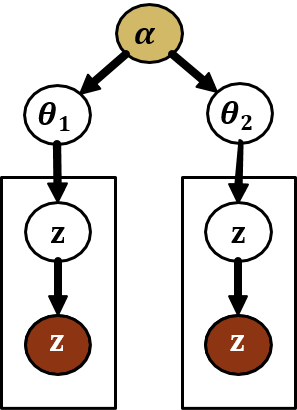
\includegraphics[scale=0.6]{fig13_11.png} 
\caption{Parametric LDA}
\label{fig:13-13}
\end{center}
\end{figure}
이번에는 Parametric LDA를 non-parametric한 형태로 바꾼 LDA에 대해 살펴보자. base distribution과 sensitivity parameter를 통해 만들어진 distribution G1과 G2으로 $\theta_{1}$, $\theta_{2}$를 만들어냈음을 볼 수 있다. 허나 여전히 이 모델은 이전 장에서 논했던 atom non-overlapping을 해결하지 못한다. 
\begin{figure}[ht] \centering 
\begin{center}
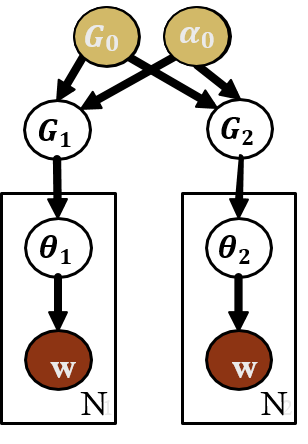
\includegraphics[scale=0.6]{fig13_12.png} 
\caption{Non-parametric LDA without Atom Sharing}
\label{fig:13-14}
\end{center}
\end{figure}

그렇다면 마지막으로 위의 atom non-overlapping 문제를 해결하는 LDA 구조에 대해 살펴보자. 먼저 $G_{0}$은 종전의 모델과 달리 H, $\gamma$의 sampling 결과로 나온 G를 쓰며 이에 따라 각 Atom의 location이 fix된 상태를 유지한다. $G_{0}$에 의해 sampling된 $G_{1}$과 $G_{2}$는 자연히 같은 Atom location을 공유하는 형태가 될 것이며 각각의 atom을 take하는 방식에 따라 cluster의 갯수나 형태를 달리하는 방식이 될 것이다.
\begin{figure}[ht] \centering 
\begin{center}
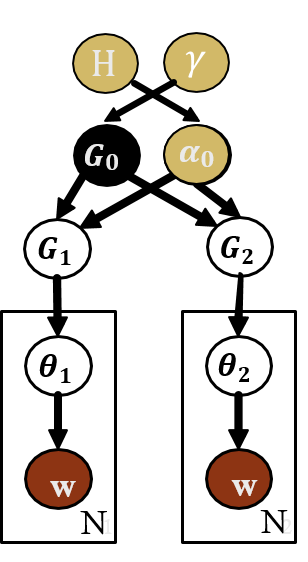
\includegraphics[scale=0.6]{fig13_13.png} 
\caption{Non-Parametric LDA with Atom Sharing}
\label{fig:13-15}
\end{center}
\end{figure}

이러한 방식이 DPMM과 비교하여 어떤 차이점을 갖는지를 생각해보자.
DPMM이 Chinese restaurant process에 의해 sampling된다고 가정하자. 이 경우 각각의 data를 assign할 때에는 이미 존재하는 table에 추가로 assign해주거나 Base distribution H에서 sampling된 $\theta$를 통해 새로운 table을 만들어 assign해주는 방식이 있었다. 

Hierarchical dirichlet process 에서 table에 각각의 data를 assign할 경우 또한 이미 존재하는 existing cluster parameter $\theta$중 일부를 다시 쓰거나, Base distribution H에서 새롭게 sampling된 new cluster parameter $\theta$를 쓰는 경우 2가지로 나눌 수 있다. 허나 HDP의 경우 이러한 $\theta$의 선택 과정에서 철저히 $G_{0}$의 영향을 받는다. 

$G_{0}$에서 sampling된 바 있는 Atom들의 location에 한하여 table이 만들어질 수 있으며, 만약 $G_{0}$에서 할당된 atom location이 아닌 곳에서 새로운 table을 만들기 위해서는 $G_{0}$에서 새로운 atom을 만들어줘야만 $G_{i}$이 새로운 atom의 location을 바탕으로 table 생성이 가능할 것이다. 즉, $G_{0}$은 마치 discrete distribution과 같은 역할을 하게 되며 $G_{i}$는 $G_{0}$의 atom에 location에서만 sampling이 가능해지는 것이다. \\

* Hierarchical structure of DIrichlet processes
\begin{center}
    H : the continuous base distribution\\
    $G_{0}$ : a draw from $G_{0}$ $\sim$ DP(H,$\gamma$)\\
    $G_{i}$ : a draw from $G_{i}$ | $G_{0}$ $\sim$ DP($G_{0}$,$\alpha_{0}$)\\
\end{center}
위의 방식을 통해서 sampling을 진행할 경우 모든 table이 $G_{0}$에 의해 이미 sampling된 바 있는 것들을 바탕으로 만들어질 것이므로 자연스럽게 atom sharing이 이루어진다고 볼 수 있다. 아래는 이에 대해 그림으로 표현한 것이다.
\begin{figure}[ht] \centering 
\begin{center}
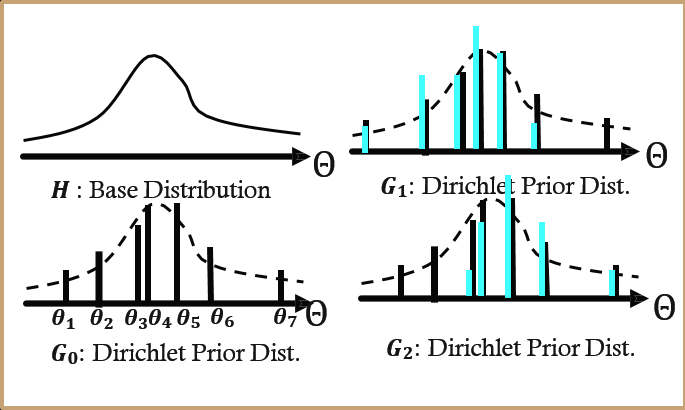
\includegraphics[scale=0.6]{fig13_14.png} 
\caption{effect of dirichlet prior distribution by Hierarchical dirichlet process}
\label{fig:13-16}
\end{center}
\end{figure}

\subsection{HDP with Stick-Breaking Construction}
%-----------------------------------------------------------------
이번에는 HDP에 Stick breaking construction이 적용된 예시에 대해 살펴보자. 먼저 $\alpha_{0}$은 테이블 각각의 값에 대한 sensitivity를 나타내며 $\gamma$의 경우 새로운 table을 얼마나 많이 만들 것인가에 대한 sensitivity parameter를 나타낸다. 마지막으로 Base distribution H는 각 table마다의 parameter를 sampling해주는 distribution이다. D는 document의 개수이며 그와 동시에 Chinese restaurant scheme의 시각에서는 restaurant의 개수라고도 칭할 수 있다. 
\begin{center}
    $G_{0} \sim DP(H,\gamma)$\\
    $G_{i}|G_{0} \sim DP(G_{0},\alpha_{0})$\\
\end{center}
이러한 관계를 식으로 더 자세히 나타내면 아래와 같이 쓸 수 있다.

* Stick breaking (prior distribution) construction of HDP
\begin{center}
    $G_{0} = \sum^{\infty}_{k=1}\beta_{k}\delta_{\phi_{k}}$\\
    $\phi_{k} \sim H $\\
    $\beta_{k} = \beta^{'}_{k}\Pi^{k-1}_{l=1}(1-\beta^{'}_{l})$\\
    $\beta^{'}_{k} | \gamma \sim Beta(1,\gamma)$\\
    $G_{i} = \sum^{\infty}_{k=1}\pi_{ik}\delta_{\phi_{k}}$\\
    $\pi_{ik} = \pi^{'}_{ik}\Pi^{k=1}_{l=1}(1-\pi^{'}_{il})$\\
    $\pi^{'}_{ik}|\alpha_{0} \sim Beta(\alpha_{0}\beta_{k},\alpha_{0}(1-\sum^{k}_{i=1}\beta_{i}))$
\end{center}
$\beta_{k}$는 개별적인 atom들이 가질 확률값을 나누는 역할을 하며 base distribution을 따르는 $\phi_{k}$는 각각의 menu와 같은 역할이라고 볼 수 있다. 

또한 $\beta_{k}$는 $\beta^{'}_{k}$을 stick breaking construction에 따라 차례대로 sampling한 값이 되며 $\beta^{'}_{k}$은 각 stick의 길이에 영향을 주는 sensitivity parameter $\gamma$에 의해 영향을 받는다. 

그 다음 $G_{i}$에 대한 식으로 넘어가보자. 식에 나타난 k의 존재를 통해 atom sharing이 성공적으로 일어나고 있음을 볼 수 있다. k에 대한 각각의 index는 모두 $G_{0}$에서 sampling된 결과를 바탕으로 하기 때문이다. $\pi_{ik}$는 $G_{0}$에 대한 식에서 $\beta_{k}$와 같은 역할을 하며 마찬가지로 $\pi^{'}_{ik}$를 stick breaking scheme으로 sampling한 각각의 값을 의미한다. 또한 위의 식에서 $\pi_{ik}$는 i번째 table에서 k번째 menu를 assign할 확률을 표현한다고도 이야기할 수 있다. 

\begin{figure}[ht] \centering 
\begin{center}
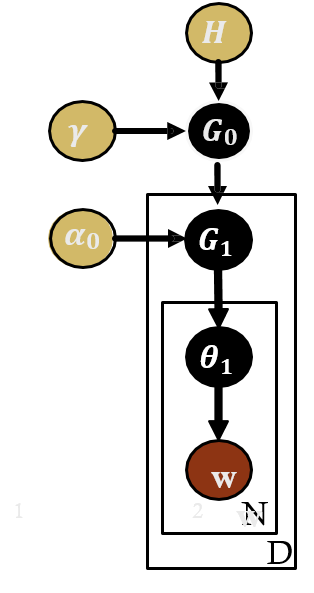
\includegraphics[scale=0.6]{fig13_15.png} 
\caption{Hierarchical dirichlet process를 기반으로 한 LDA}
\label{fig:13-17}
\end{center}
\end{figure}

\subsection{Chinese Restaurant Franchise}
%-----------------------------------------------------------------
앞에서 배운 내용들을 정리하여 Chinese Restaurant Franchise라는 넓은 개념을 정의해보도록 하겠다. 
\begin{center}
    $G_{0} \sim DP(H,\gamma)$\\
    $G_{i}|G_{0} \sim DP(G_{0},\alpha_{0})$\\
\end{center}
결국 $G_{0}$은 Chinese Restaurant Franchise 관점에서 각각의 Menu를 만들어내는 과정이며 $G_{i}$은 $G_{0}$가 만들어놓은 Menu들을 바탕으로 각각의 table을 만들어내는 과정이라 할 수 있다.  결국 각각의 table은 menu와 associative한 관계에 있는 것이다. 
\begin{center}
    $\theta_{in} \sim G_{i}$ : a $\theta_{in}$'s seating on a $\Psi_{it}$ table of each restaurant\\
    $\phi_{k} \sim G_{0}$ : a $\Psi_{it}$'s table serves a $\phi_{k}$ menu of the franchise
\end{center}
또한 $\theta_{in}$는 $G_{i}$에 의해 sampling된 값으로서 각 cluster에 대한 parameter를 의미한다. 또한 i번째 restaurant의 n번째 word가 $\Psi_{it}$ table에 앉게 되는 것을 의미하는 값이기도 한다. 그렇다면 $\Psi_{it}$는 무엇인가? 

$\Psi_{it}$는 각각의 table이 생겨날 때마다 자동적으로 생성되는 값으로서 i번째 restaurant의 t번째 table이 $\phi_{k}$번째 menu를 serve하는 것을 의미하는 값이기도 하다. 이를 graphical하게 표현하면 아래와 같다.

\begin{figure}[ht] \centering 
\begin{center}
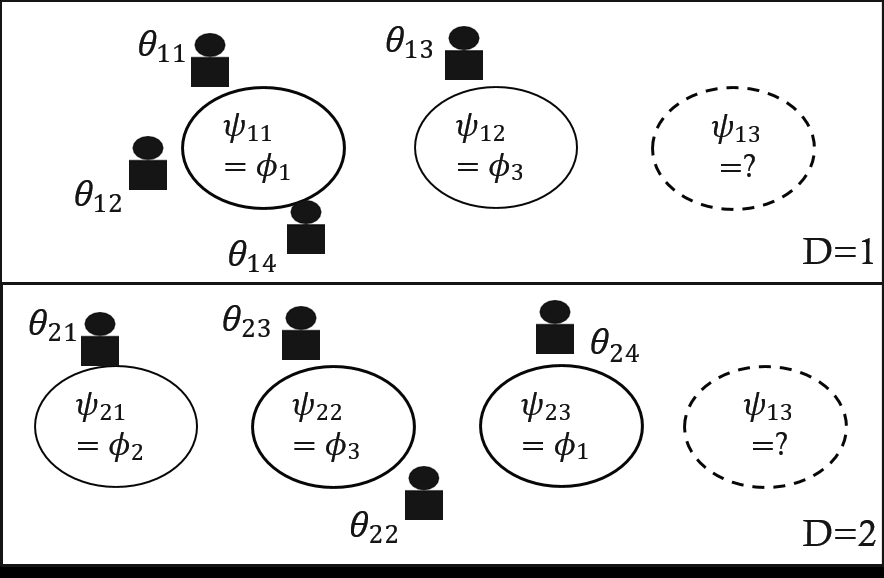
\includegraphics[scale=0.6]{fig13_16.png} 
\caption{table view of Chinese Restaurant Franchise}
\label{fig:13-18}
\end{center}
\end{figure}
원래 Chinese restaurant scheme에서는 새로운 table을 만들 때 마다 base distribution에서 임의의 값을 sampling하여 나온 cluster parameter $\theta$를 사용하였다. 하지만 Chinese restaurant Franchise의 상황에선 위의 그림과 같이  $\theta$ 대신 각각의 table마다 $\Psi$를 생성한 다음 $\Psi$에 assign해줄 수 있는 값으로 $G_{0}$에서 만들어진 atom 후보군 $\phi$중의 하나를 sampling하게 된다. 

위의 그림을 예시로 들어보자. D=1, 즉 첫번째 restaurant에서 $\theta_{11}$과 $\theta_{12}$와 달리 $\theta_{13}$은 새로운 table을 만들었다. 이에 따라 $\Psi_{12}$가 생성되었고 이에 assign될 menu 단계에서의 값이 $\Phi_{3}$로 선택되었음을 알 수 있다. 

이처럼 Chinese Restaurant Franchise (CRF)의 CRP sampling은 2단 구조로 이루어지고 있다. $\theta$와 $\Psi$간의 sampling이 기존에서도 일어나던 table에 대한 sampling이라면 CRF에서는 각 table의 menu에 대한 sampling이 한 차례 더 일어나고 있음을 아래의 그림을 통해 확인할 수 있다. 

\begin{figure}[ht] \centering 
\begin{center}
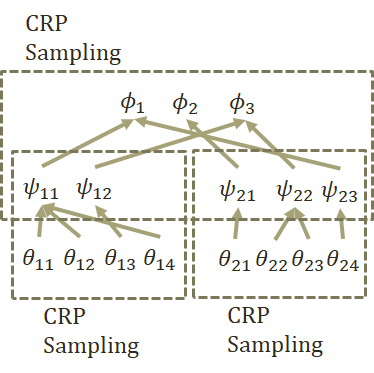
\includegraphics[scale=0.5]{fig13_17.png} 
\caption{Hierarchical structure of CRP sampling}
\label{fig:13-19}
\end{center}
\end{figure}

이러한 sampling 방식을 Gibb's sampling으로 바꾸려면 어떻게 해야할까? 먼저 de Finetti's theorem을 이용하여 모든 data에 대한 assignment가 되어 있음을 가정한 후에 특정 data를 다시 sampling 하는 방식을 취해야할 것이다. 이 경우 해당 data의 assignment가 일시적으로 없어짐에 따라 해당 table또한 함께 없어질 수 있는데, 이에 따라 해당 table $\Psi$의 정보를 없애주고 해당 table이 선택한 menu $\Phi$의 count 또한 줄여준 이후에 sampling이 이루어져야 할 것이다. 만약 채택된 menu가 assign된 모든 table이 없어질 경우 해당 menu $\Phi$ 또한 마찬가지로 없애주어야 할 것이다. 


\end{document}








































































































































































































































































































































































































































































































































































































































































































































































































































































































































































































































































































































































































































































































































































































































































































































































































































































































































































































































































































































































































































































































































































































































































































































































































































































































































































































































































































































































































































































































































































































































































































































































































































































































































































































































































































































































































































































































































































































































































































































































































































































































































































































































































































